\documentclass[]{elementary-physics}

\title{2. Increasing Momentum or Charge}
\date{2015-05-11 v4.9}

\begin{document}

\maketitle

\tableofcontents

\section{Abstract}

When a mass collide elastically into a bigger mass so that the mass bounce and velocity change sign the sum of the absolute of the momentum in the system increase.
The same can be done with capacitors in series with an inductor with respect to charge.

\section{Increasing Absolute Momentum}

As an example we will use one mass of $2 kg$ with velocity $1 m/s$ and one mass of $3 kg$ with zero velocity:

\begin{figure}[ht] \centering
	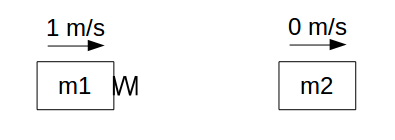
\includegraphics[scale=.5]{mms4} \caption{Masses initial state}
\end{figure}

\begin{subequations}
\begin{align}
m_1 &= 2 \, kg \\
v_1 &= 1 \, m/s \\
p_1 &= 2 \, kg \, m/s \\
m_2 &= 3 \, kg \\
v_2 &= 0 \, m/s \\
p_2 &= 0 \, kg \, m/s
\end{align}
\end{subequations}

Masses in a collision are combined in parallel\cite{ef1ch} so we calculate the properties of the combination:

\begin{subequations}
\begin{align}
m_c &= 1/(1/2 + 1/3) = 1.2 \, kg \\
v_c &= 1 - 0 = 1 \, m/s \\
p_c &= 1.2 * 1 = 1.2 \, kg \, m/s
\end{align}
\end{subequations}

To calculate the resulting velocity for a totally inelastic collision we either subtract the momentum of the combination from $m_1$ or add it to $m_2$ and then calculate the new velocity from that:

\begin{figure}[ht] \centering
	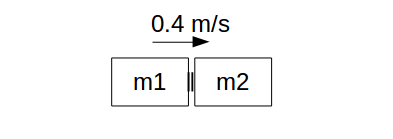
\includegraphics[scale=.5]{mms5} \caption{Masses inelastic collision}
\end{figure}

\begin{subequations}
\begin{align}
m_1 &= 2 \, kg \\
p_1 &= 2 - 1.2 = 0.8 \, kg \, m/s \\
v_1 &= 0.8 / 2 = 0.4 \, m/s \\
m_2 &= 3 \, kg \\
p_2 &= 0 + 1.2 = 1.2 \, kg \, m/s \\
v_2 &= 1.2 / 3 = 0.4 \, m/s
\end{align}
\end{subequations}

The sum of the momentums is the same as before the inelastic collision:

\begin{equation}
\sum p = 0.8 + 1.2 = 2 \, kg \, m/s
\end{equation}

To calculate the resulting velocity for an elastic collision we subtract the momentum of the combination twice from $m_1$ and add it twice to $m_2$ and then calculate the new velocities from that:

\begin{figure}[ht] \centering
	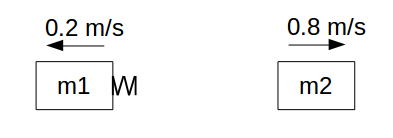
\includegraphics[scale=.5]{mms6} \caption{Masses elastic collision}
\end{figure}

\begin{subequations}
\begin{align}
m_1 &= 2 \, kg \\
p_1 &= 2 - 2*1.2 = -0.4 \, kg \, m/s \\
v_1 &= -0.4 / 2 = -0.2 \, m/s \\
m_2 &= 3 \, kg \\
p_2 &= 0 + 2*1.2 = 2.4 \, kg \, m/s \\
v_2 &= 2.4 / 3 = 0.8 \, m/s
\end{align}
\end{subequations}

The sum of the momentums is the same as before the elastic collision:

\begin{equation}
\sum p = -0.4 + 2.4 = 2 \, kg \, m/s
\end{equation}

But the sum of the absolute of the momentums has changed:

\begin{equation}
\sum | p | = 0.4 + 2.4 = 2.8 > 2 \, kg \, m/s
\end{equation}

As You can see, $\sum p$ is conserved, but $\sum | p |$ has increased.
The momentum after the elastic collision is in fact greater even if $m_1$ would be removed altogether:

\begin{equation}
p_2 = 2.4 > 2 \, kg \, m/s
\end{equation}

Kinetic energy is of course constant.
 
\section{Increasing Absolute Charge}

The same thing will happen value-wise if we instead have two capacitors and an inductor.

\begin{figure}[ht] \centering
	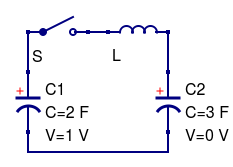
\includegraphics[scale=.5]{ccl7} \caption{Capacitors initial state}
\end{figure}

The sum of the charge is initially $2 C$.

\begin{figure}[ht] \centering
	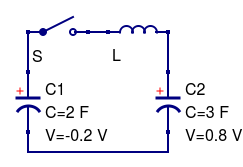
\includegraphics[scale=.5]{ccl8} \caption{Capacitors after 'elastic collision'}
\end{figure}

The sum of the absolute of the charge is $2.8 C$ after the 'collision'.

\begin{figure}[ht] \centering
	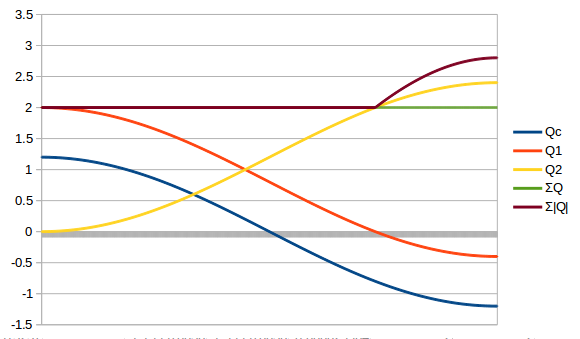
\includegraphics[scale=.5]{cclg} \caption{Charge during 'elastic collision'}
\end{figure}

The sum of the absolute of the charges starts to increase just as $q_1$ goes negative.

\section{Repeated Elastic Collisions}

Assuming $m_1<<m_2$ and the following initial velocities:

\begin{subequations}
\begin{align}
v_1 &= {v_1}_{max} \\
v_2 &= 0
\end{align}
\end{subequations}

then if we change the sign of $v_1$ after a collision, collisions can be repeated.
Since kinetic energy is constant we will eventually have:

\begin{subequations}
\begin{align}
v_1 &= 0 \\
v_2 &= {v_2}_{max} \\
\frac{m_1 \, {v_1}_{max}^2}{2} &= \frac{m_2 \, {v_2}_{max}^2}{2}
\end{align}
\end{subequations}

If we set

\begin{equation}
K = \sqrt{\frac{m_2}{m_1}}
\end{equation}

then

\begin{equation}
\frac{{v_1}_{max}}{{v_2}_{max}} = \frac{{p_2}_{max}}{{p_1}_{max}} = K
\end{equation}

If the path of the masses is circular, and $n$ is the number of collisions performed, we have:

\begin{subequations}
\begin{align}
m &= \frac{m_1 m_2}{m_1 + m_2} \\
v(n) &= v_1(n) - v_2(n) \\
p(n) &= m \, v(n) \\
v_1(n+1) &= -\frac{m_1 v_1(n) - 2p(n)}{m_1} \\
v_2(n+1) &= \frac{m_2 v_2(n) + 2p(n)}{m_2} \\
v_1(0) &= {v_1}_{max} \\
v_2(0) &= 0
\end{align}
\end{subequations}

then the momentum of the system will oscillate between ${p_2}_{max}$ and $-{p_2}_{max}$:

\begin{subequations}
\begin{align}
%\frac{{v_1}_{max}}{{v_2}_{max}} &= K \\
f &= \frac{1}{\pi K} \\
v_1(n) &= {v_1}_{max} \cos (\frac{2n}{K}) \\
v_2(n) &= {v_2}_{max} \sin (\frac{2n}{K})
\end{align}
\end{subequations}

$v_1(n)$ can also be described as an differential equation:

\begin{subequations}
\begin{align}
m_2 v_1''(n) + 4 m_1 v_1(n) &= 0 \\
v_1(0) &= {v_1}_{max}
\end{align}
\end{subequations}

But in the end, as stated above, it all boils down to:

\begin{subequations}
\begin{align}
p &= m v\\
E &= \frac{m v^2}{2}
\end{align}
\end{subequations}

where $E$ is constant and transferred from $m_1$ to $m_2$ (back and forth).
If mass, from $E$'s point of view, is increased by a factor $z=m_2/m_1$ then $v$ has to be decreased by factor $\sqrt{z}=K$ and so $p$ is increased by factor $K$:

\begin{subequations}
\begin{align}
E &= \frac{z\,m \left( \frac{v}{\sqrt{z}} \right)^2}{2} \\
p &= z\,m \frac{v}{\sqrt{z}} = \sqrt{z}\,m v = K\,m v \\
\end{align}
\end{subequations}

The same can of course be done with two capacitors and an inductor.

\pagebreak

\section{Experiment}

In an experiment the following components where used;

\begin{subequations}
\begin{align}
C_1 &= 1 \, \mu F \\
V_1 &= 32 \, V \\
Q_1 &= 32 \, \mu C \\
E_1 &= 512 \, \mu J \\
C_2 &= 47 \, \mu F \\
V_2 &= 0 \, V \\
Q_2 &= 0 \, C \\
E_2 &= 0 \, J
\end{align}
\end{subequations}

\begin{figure}[ht] \centering
	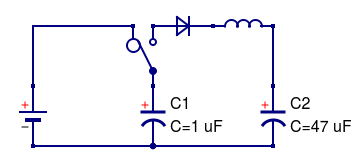
\includegraphics[scale=.5]{BLCC} \caption{Experiment}
\end{figure}

After several attempts where it seemed like the switch was bouncing and distorting the results the switch was turned and the following measurements was noted:

\begin{subequations}
\begin{align}
C_1 &= 1 \, \mu F \\
V_1 &= -16 \, V \\
Q_1 &= -16 \, \mu C \\
E_1 &= 128 \, \mu J \\
C_2 &= 47 \, \mu F \\
V_2 &= 1 \, V \\
Q_2 &= 47 \, \mu C \\
E_2 &= 24 \, \mu J
\end{align}
\end{subequations}

Although the voltmeter was quickly draining $C_1$ enough voltage was left to show that absolute charge had increased.

\begin{subequations}
\begin{align}
\sum Q_{old} &= 32 \, \mu C \\
\sum Q_{new} &= 31 \, \mu C \\
\sum |Q_{new}| &= 63 \, \mu C
\end{align}
\end{subequations}

Had there been no losses we would have had:

\begin{subequations}
\begin{align}
C_1 &= 1 \, \mu F \\
V_1 &= -30.67 \, V \\
Q_1 &= -30.67 \, \mu C \\
E_1 &= 470.22 \, \mu J \\
C_2 &= 47 \, \mu F \\
V_2 &= 1.33 \, V \\
Q_2 &= 62.67 \, \mu C \\
E_2 &= 41.78 \, \mu J \\
\sum |Q_{new}| &= 93.33 \, \mu C
\end{align}
\end{subequations}

Watch the experiment at \url{https://www.youtube.com/watch?v=xZcvOWSXcbU}.

\section{Conclusion}

Although $\sum p$ and $\sum E$ in a closed system are always constant for masses, two \textit{Conservations Laws}, $\sum | p |$ is not, just as $\sum Q$ is always constant for capacitors, another \textit{Conservation Law}, but $\sum | Q |$ is not.
By e.g flipping one of the capacitors for each cycle, or enclose it in a full-wave bridge-rectifier, the charge can be transferred efficiently from a small capacitor to a big.
This is also the case for springs and inductors, but they may need a paper on its own.

\appendix

\section{In Plain English}

In a closed system is the sum of the momentums before a collision is always the same as the sum of the momentum after the collision.
But if one and only one of the colliding masses in a one-dimensional system change direction of movement as a result of the collision the sum of the absolute value of the momentums change.
Similarly, the sum of the charges in a system with two capacitors and a coil in series is constant.
However, if the voltage in one and only one of the capacitors change polarity the sum of the absolute value of the charges in the system change.

As an example, a small mass of $1 kg$ with a momentum of $10 kgm/s$ collide with a larger stationary mass of $19 kg$ and bounce back with momentum of $-9 kgm/s$.
The greater mass must now have a momentum of $19 kgm/s$ for the sum of the momentums to be constant.
After the collision, the system's momentum has increased from $10 kgm/s$ to $19 kgm/s$ if we do not take the small mass into account.
If we include the absolute value of the momentum of the small mass the system momentum has increased from $10 kgm/s$ to $28 kgm/s$.
The kinetic energy is constant at $50 J$.

\section{På Ren Svenska}

I ett slutet system är summan av rörelsemängderna före en kollision alltid densamma som summan av rörelsemängderna efter kollisionen.
Men om en och endast en av de kolliderande massorna i ett endimensionellt system byter rörelseriktning som ett resultat av kollisionen så har summan av absolutvärdet av rörelsemängderna ändrats.
På samma sätt gäller det att summan av laddningarna i ett  system med två kondensatorer och en spole i serie är konstant.
Men om spänningen i en och endast en av kondensatorerna växlar polaritet så ändras summan av absolutvärdet av laddningarna i systemet.

Som ett exempel, en liten massa på $1 kg$ med rörelsemängden $10 kgm/s$ kollisiderar med en större stillastående massa på $19 kg$ och studsar tillbaka med rörelsemängden $-9 kgm/s$.
Den större massan måste nu ha en rörelsemängd på $19 kgm/s$ för att summan av rörelsemängderna skall vara konstant.
Efter kollisionen har systemets rörelsemängd ökat från $10 kgm/s$ till $19 kgm/s$ om vi inte räknar med den lilla massan.
Om vi räknar med absolutvärdet av den lilla massans rörelsemängd har systemets rörelsemängd ökat från $10 kgm/s$ till $28 kgm/s$.
Rörelseenergin är konstant $50 J$.

\section{This Paper}

This is one paper from a collection of papers, all free to be downloaded and shared. If you have ideas how to enhance any of the papers, if you want to contribute, don’t hesitate to contact us at \url{hob.nilre@gmail.com}.\\
\\
The papers can all be found at:
\begin{itemize}
\item \url{https://sites.google.com/site/nilrehob/home/elementary-physics}
\item \url{https://independent.academia.edu/HobNilre/Papers}
\item \url{https://groups.yahoo.com/neo/groups/EVGRAY/files/Hob/}
\item \url{http://overunity.com/15796/elementary-physics-revisited/}
\item \url{http://idipsum.se/home/elementary%20physics.html}
\item \url{https://github.com/boherlin/elementary-physics/tree/master/pdf}
\end{itemize}

They are updated with new versions in an unpredictable manner, possibly not on all sites but at least on the last two sites in the list, make sure you always have the latest version!
Their \LaTeX source-codes can be found at \url{https://github.com/boherlin/elementary-physics/tree/master/src}.
All papers, but not all versions, have been stamped at \url{http://www.OriginStamp.org}.\\
\\
If you enjoyed this paper, found value in it and want to help us, please consider giving us a donation in bitcoin, this is our address:

\begin{figure}[ht] \centering
	
\includegraphics[]{1B79p75vQw4Rb1GQdmGYpDapFwEytFJDqw} \caption{1B79p75vQw4Rb1GQdmGYpDapFwEytFJDqw}
\end{figure}


\printbibliography

\end{document}
